\documentclass[12pt,spanish,fleqn,openany,letterpaper,pagesize]{scrbook}
\usepackage[ansinew]{inputenc}
\usepackage[spanish]{babel}
\usepackage{fancyhdr}
\usepackage{epsfig}
\usepackage{epic}
\usepackage{eepic}
\usepackage{amsmath}
\usepackage{threeparttable}
\usepackage{amscd}
\usepackage{here}
\usepackage{graphicx}
\usepackage{lscape}
\usepackage{tabularx}
\usepackage{subfigure}
\usepackage{longtable}
\usepackage{rotating} 
\renewcommand{\theequation}{\thechapter-\arabic{equation}}
\renewcommand{\thefigure}{\textbf{\thechapter-\arabic{figure}}}
\renewcommand{\thetable}{\textbf{\thechapter-\arabic{table}}}


\pagestyle{fancyplain}%\addtolength{\headwidth}{\marginparwidth}
\textheight22.5cm \topmargin0cm \textwidth16.5cm
\oddsidemargin0.5cm \evensidemargin-0.5cm%
\renewcommand{\chaptermark}[1]{\markboth{\thechapter\; #1}{}}
\renewcommand{\sectionmark}[1]{\markright{\thesection\; #1}}
\lhead[\fancyplain{}{\thepage}]{\fancyplain{}{\rightmark}}
\rhead[\fancyplain{}{\leftmark}]{\fancyplain{}{\thepage}}
\fancyfoot{}
\thispagestyle{fancy}%
\addtolength{\headwidth}{0cm}
\unitlength1mm %Define la unidad LE para Figuras
\mathindent0cm %Define la distancia de las formulas al texto,  fleqn las descentra
\marginparwidth0cm
\parindent0cm %Define la distancia de la primera linea de un parrafo a la margen

%Para tablas,  redefine el backschlash en tablas donde se define la posici\'{o}n del texto en las
%casillas (con \centering \raggedright o \raggedleft)
\newcommand{\PreserveBackslash}[1]{\let\temp=\\#1\let\\=\temp}
\let\PBS=\PreserveBackslash

%Espacio entre lineas
\renewcommand{\baselinestretch}{1.1}

%Neuer Befehl f\"{u}r die Tabelle Eigenschaften der Aktivkohlen
\newcommand{\arr}[1]{\raisebox{1.5ex}[0cm][0cm]{#1}}

%Neue Kommandos
\usepackage{Befehle}
%Trennungsliste
\hyphenation {Reaktor-ab-me-ssun-gen Gas-zu-sa-mmen-set-zung
Raum-gesch-win-dig-keit Durch-fluss Stick-stoff-gemisch
Ad-sorp-tions-tem-pe-ra-tur Klein-schmidt
Kohlen-stoff-Mole-kular-siebe Py-rolysat-aus-beu-te
Trans-port-vor-gan-ge}
%\includeonly{Kap1/Kap1,Kap2/Kap2}
\begin{document}
\pagenumbering{roman}
%\newpage
%\setcounter{page}{1}
\begin{center}
\begin{figure}
\centering%
%
\epsfig{file=HojaTitulo/University_of_Los_Andes_logo.xvg,scale=1}%

\includegraphics[scale=0.2]{./HojaTitulo/University_of_Los_Andes_logo.pdf}
\end{figure}
\thispagestyle{empty} \vspace*{1.5cm} \textbf{\huge
Simulaciones por Din\'{a}mica Molecular para el Estudio de Propiedades Biof\'{i}sicas de Estafiloxantina en Membranas Modelo de \textit{Staphylococcus aureus}}\\[5.0cm]
\Large\textbf{John Erick Cabrera Ramirez}\\[6.0cm]
\small Universidad de los Andes\\
Facultad de Ciencias, Departamento de F\'{i}sica\\
Bogot\'{a}, Colombia\\
%A\~{n}o\\
2020\\
\end{center}

\newpage{\pagestyle{empty}\cleardoublepage}

\newpage
\begin{center}
\thispagestyle{empty} \vspace*{-1cm} \textbf{\huge
Simulaciones por Din\'{a}mica Molecular para el Estudio de Propiedades Biof\'{i}sicas de Estafiloxantina en Membranas Modelo de \textit{Staphylococcus aureus}}\\[3.0cm]
\Large\textbf{John Erick Cabrera Ramirez}\\[3.0cm]
\small Tesis o trabajo de grado presentada(o) como requisito parcial para optar al
t\'{\i}tulo de:\\
\textbf{Mag\'{i}ster en Ciencias-F\'{i}sica}\\[2.0cm]
Director(a):\\
%T\'{\i}tulo (Ph.D., Doctor, Qu\'{\i}mico, etc.) y nombre del director(a)\\[2.0cm]
Ph. D. Chad Leidy\\[2.0cm]
L\'{\i}nea de Investigaci\'{o}n:\\
%Nombrar la l\'{\i}nea de investigaci\'{o}n en la que enmarca la tesis  o trabajo de investigaci\'{o}n\\
Biof\'{i}sica de membranas\\
%Grupo de Investigaci\'{o}n:\\
%Biof\'{i}sica de membranas\\
[2.5cm]
Universidad de los Andes\\
Facultad de Ciencias, Departamento de F\'{i}sica\\
Bogot\'{a}, Colombia\\
%A\~{n}o\\
2020\\
\end{center}

\newpage{\pagestyle{empty}\cleardoublepage}

\newpage
\thispagestyle{empty} \textbf{}\normalsize
\\\\\\%
\textbf{(Dedicatoria o un lema)}\\[4.0cm]

\begin{flushright}
\begin{minipage}{8cm}
    \noindent
        \small
        Su uso es opcional y cada autor podr\'{a} determinar la distribuci\'{o}n del texto en la p\'{a}gina, se sugiere esta presentaci\'{o}n. En ella el autor dedica su trabajo en forma especial a personas y/o entidades.\\[1.0cm]\\
        Por ejemplo:\\[1.0cm]
        A mis padres\\[1.0cm]\\
        o\\[1.0cm]
        La preocupaci\'{o}n por el hombre y su destino siempre debe ser el
        inter\'{e}s primordial de todo esfuerzo t\'{e}cnico. Nunca olvides esto
        entre tus diagramas y ecuaciones.\\\\
        Albert Einstein\\
\end{minipage}
\end{flushright}

\newpage{\pagestyle{empty}\cleardoublepage}

\newpage
\thispagestyle{empty} \textbf{}\normalsize
\\\\\\%
\textbf{\LARGE Agradecimientos}
\addcontentsline{toc}{chapter}{\numberline{}Agradecimientos}\\\\
Esta secci\'{o}n es opcional, en ella el autor agradece a las personas o instituciones que colaboraron en la realizaci\'{o}n de la tesis  o trabajo de investigaci\'{o}n. Si se incluye esta secci\'{o}n, deben aparecer los nombres completos, los cargos y su aporte al documento.\\

\newpage{\pagestyle{empty}\cleardoublepage}

\newpage
\textbf{\LARGE Resumen}
\addcontentsline{toc}{chapter}{\numberline{}Resumen}\\\\
El resumen es una presentaci\'{o}n abreviada y precisa (la NTC 1486 de 2008 recomienda revisar la norma ISO 214 de 1976). Se debe usar una extensi\'{o}n m\'{a}xima de 12 renglones. Se recomienda que este resumen sea anal\'{\i}tico, es decir, que sea completo, con informaci\'{o}n cuantitativa y cualitativa, generalmente incluyendo los siguientes aspectos: objetivos, dise\~{n}o, lugar y circunstancias, pacientes (u objetivo del estudio), intervenci\'{o}n, mediciones y principales resultados, y conclusiones. Al final del resumen se deben usar palabras claves tomadas del texto (m\'{\i}nimo 3 y m\'{a}ximo 7 palabras), las cuales permiten la recuperaci\'{o}n de la informaci\'{o}n.\\

\textbf{\small Palabras clave: (m\'{a}ximo 10 palabras, preferiblemente seleccionadas de las listas internacionales que permitan el indizado cruzado)}.\\

A continuaci\'{o}n se presentan algunos ejemplos de tesauros que se pueden consultar para asignar las palabras clave, seg\'{u}n el \'{a}rea tem\'{a}tica:\\

\textbf{Artes}: AAT: Art y Architecture Thesaurus.

\textbf{Ciencias agropecuarias}: 1) Agrovoc: Multilingual Agricultural Thesaurus - F.A.O. y 2)GEMET: General Multilingual Environmental Thesaurus.

\textbf{Ciencias sociales y humanas}: 1) Tesauro de la UNESCO y 2) Population Multilingual Thesaurus.

\textbf{Ciencia y tecnolog\'{\i}a}: 1) Astronomy Thesaurus Index. 2) Life Sciences Thesaurus, 3) Subject Vocabulary, Chemical Abstracts Service y 4) InterWATER: Tesauro de IRC - Centro Internacional de Agua Potable y Saneamiento.

\textbf{Tecnolog\'{\i}as y ciencias m\'{e}dicas}: 1) MeSH: Medical Subject Headings (National Library of Medicine's USA) y 2) DECS: Descriptores en ciencias de la Salud (Biblioteca Regional de Medicina BIREME-OPS).

\textbf{Multidisciplinarias}: 1) LEMB - Listas de Encabezamientos de Materia y 2) LCSH- Library of Congress Subject Headings.\\

Tambi\'{e}n se pueden encontrar listas de temas y palabras claves, consultando las distintas bases de datos disponibles a trav\'{e}s del Portal del Sistema Nacional de Bibliotecas\footnote{ver: www.sinab.unal.edu.co}, en la secci\'{o}n "Recursos bibliogr\'{a}ficos" opci\'{o}n "Bases de datos".\\

\textbf{\LARGE Abstract}\\\\
Es el mismo resumen pero traducido al ingl\'{e}s. Se debe usar una extensi\'{o}n m\'{a}xima de 12 renglones. Al final del Abstract se deben traducir las anteriores palabras claves tomadas del texto (m\'{\i}nimo 3 y m\'{a}ximo 7 palabras), llamadas keywords. Es posible incluir el resumen en otro idioma diferente al espa\~{n}ol o al ingl\'{e}s, si se considera como importante dentro del tema tratado en la investigaci\'{o}n, por ejemplo: un trabajo dedicado a problemas ling\"{u}\'{\i}sticos del mandar\'{\i}n seguramente estar\'{\i}a mejor con un resumen en mandar\'{\i}n.\\[2.0cm]
\textbf{\small Keywords: palabras clave en ingl\'{e}s(m\'{a}ximo 10 palabras, preferiblemente seleccionadas de las listas internacionales que permitan el indizado cruzado)}\\

\renewcommand{\tablename}{\textbf{Tabla}}
\renewcommand{\figurename}{\textbf{Figura}}
\renewcommand{\listtablename}{Lista de Tablas}
\renewcommand{\listfigurename}{Lista de Figuras}
\renewcommand{\contentsname}{Contenido}


%\newcommand{\clearemptydoublepage}{\newpage{\pagestyle{empty}\cleardoublepage}}
\tableofcontents
\chapter*{Lista de s\'{\i}mbolos}
\addcontentsline{toc}{chapter}{\numberline{}Lista de s\'{\i}mbolos}
\section*{S\'{\i}mbolos con letras latinas}
 \label{simbolos}
 %\renewcommand{\arraystretch}{3}
\begin{longtable}{p{2cm}p{4cm}p{2cm}p{8cm}}
\textbf{S\'{\i}mbolo}&\textbf{T\'{e}rmino}&\textbf{Unidad SI}&\textbf{Definici\'{o}n}\\[0.5ex]\hline
\endfirsthead%
\textbf{S\'{\i}mbolo}&\textbf{T\'{e}rmino}&\textbf{Unidad SI}&\textbf{Definici\'{o}n}\\[0.5ex]\hline
\endhead%
      $Z$&N\'{u}mero at\'{o}mico&\hspace{6pt}1&N\'{u}mero de protones en un \'{a}tomo\\%
      pH &Potencial de hidr\'{o}geno &\hspace{6pt}1&Grado de acidez o alcanilidad en una soluci\'{o}n\\%
      $r_{ij}$&Distancia entre part\'{i}culas $i$ y $j$&\hspace{6pt}m&Secci\'{o}n \ref{ssec:Estruc}\\%
      e&Carga del electr\'{o}n&\hspace{6pt}A.s&$e=1.602\times 10^{19}$C\\%
\ce{P_{1}}&Sistema tricl\'{i}nico&\hspace{6pt}-&Secci\'{o}n \ref{sec:esvSGLT}\\%
\ce{P_{21}}&Sistema monocl\'{i}nico&\hspace{6pt}-&Secci\'{o}n \ref{sec:esvSGLT}\\
\ce{P_{21}P_{21}P_{21}}&Sistema ortorr\'{o}mbico&\hspace{6pt}-&Secci\'{o}n \ref{sec:esvSGLT}\\
$V$ &Energ\'{i}a potencial&\hspace{6pt}J&Forma de energ\'{i}a que depende de la posici\'{o}n o una propiedad del objeto\\%
$T$&Energ\'{i}a cin\'{e}tica&\hspace{6pt}J&Forma de energ\'{i}a que depende de la velocidad de un objeto\\%
$E$  &Energ\'{i}a total&\hspace{6pt}J&Suma de las formas de energ\'{i}a\\%
$q$&Coordenada generalizada&\hspace{6pt}-&Par\'{a}metro que representa la configuraci\'{o}n del sistema respecto a una referencia.\\%
$N$&N\'{u}mero de part\'{i}culas&\hspace{6pt}1&N\'{u}mero de part\'{i}culas\\%
$\frac{\partial}{\partial q_i}$&Derivada parcial&\hspace{6pt}-&Raz\'{o}n de cambio instant\'{a}nea respecto a la coordenada $q_i$\\%
$\mathbf{A}$&Matriz A (en negrita)&\hspace{6pt}-&$\mathbf{A}=\{a_{ij}\}$\\%
$\mathbf{r_i}$&Vector de posici\'{o}n part\'{i}cula $i$&\hspace{6pt}m&$\mathbf{r_i}=\left(x_i,y_i,z_i\right)$\\%
$\mathbf{M}$&Matriz de masa del sistema&\hspace{6pt}kg&Secci\'{o}n \ref{sec:MecNMA}\\%
$\mathbf{U}$&Matriz de constantes el\'{a}sticas&\hspace{6pt}N/m&Ecuaci\'{o}n \eqref{eq:5}\\%
$\mathbf{r}$&Coordenadas de masa ponderada para la posici\'{o}n&\hspace{6pt}$\mathrm{m.kg^{1/2}}$ &Ecuaciones \eqref{eq:15}\\%
$\mathbf{K}$&Constantes el\'{a}sticas en las coordenadas ponderadas&\hspace{6pt}$\mathrm{N/kg.m}$ &Ecuaciones \eqref{eq:15}\\%
$\lambda_k$&Autovalor $k$\'{e}simo &\hspace{6pt}$\mathrm{rad^2/s^2}$&Ecuaci\'{o}n \eqref{eq:18}\\%
$\mathbf{a_k}$&Autovector correspondiente a $\lambda_k$&\hspace{6pt}$\mathrm{m.kg^{1/2}}$ &Ecuaci\'{o}n \eqref{eq:18}\\%
$\zeta_k$   &Coordenada normal correspondiente a $\omega_k$&\hspace{6pt}1 &Ecuaci\'{o}n \eqref{eq:nor}\\%
$E_s$&Energ\'{i}a del sistema &\hspace{6pt}J  &Suma de las formas de energ\'{i}a\\%
$k_B$&Constante de Boltzmann &\hspace{6pt}J/K&$k_B=1.38\times 10^{-23}$J/K\\%
$p$&Densidad de probabilidad &\hspace{6pt}1 &Probabilidad por unidad de volumen del espacio de fase\\%
$Z$  &Funci\'{o}n de partici\'{o}n&\hspace{6pt}1 &Probabilidad por unidad de volumen del espacio de fase\\%
$T$ &Temperatura &\hspace{6pt}K &Es una mediad objetiva de que tan caliente o fr\'{i}o\\%
$H(\mathbf{p},\mathbf{q})$ &Hamiltoniano  &\hspace{6pt}J &Transformada de Legendre del Lagrangiano\\%
$n$ &N\'{u}mero de coordenadas    &\hspace{6pt}1 &$n=3N$\\%
$n$&N\'{u}mero de coordenadas   &\hspace{6pt}1 &$n=3N$\\%
$\prod_i^m x_i$&Productoria&\hspace{6pt}-&$\prod_i^m x_i=x_1x_2...x_m$\\%
$\hbar$&Constante de Plank reducida &\hspace{6pt}J.s &$\hbar=\frac{h}{2\pi}=1.054\times 10^{-34}$J.s\\%
$R_{ij}^0$&Distancia de equilibrio entre los nodos $i$ y $j$ &\hspace{6pt}m&Secci\'{o}n \ref{ssec:ANM}\\%
$R_{ij}$&Distancia entre los nodos $i$ y $j$ &\hspace{6pt}m&Secci\'{o}n \ref{ssec:ANM}\\%
\end{longtable}
\vspace{10ex}
\section*{S\'{\i}mbolos con letras griegas}

\begin{longtable}{p{2cm}p{3.5cm}p{2cm}p{8cm}}
\textbf{S\'{\i}mbolo}&\textbf{T\'{e}rmino}&\textbf{Unidad SI}&\textbf{Definici\'{o}n}\\[0.5ex] \hline%
\endfirsthead%
\textbf{S\'{\i}mbolo}&\textbf{T\'{e}rmino}&\textbf{Unidad SI}&\textbf{Definici\'{o}n}\\[0.5ex] \hline%
\endhead%
\renewcommand{\arraystretch}{1.3}
 \label{simbolosg}
 $(\phi,\psi,\omega)$&\'{A}ngulos diedros&\hspace{6pt}rad &Secci\'{o}n \\
  $\epsilon_0$&Permitividad en el vac\'{i}o&\hspace{6pt}$\mathrm{C^2/N.m^2}$&$\epsilon_0=8.85\times 10^{-12}\mathrm{C^2/N.m^2}$ \\ 
   $\epsilon_r$&Permitividad relativa&\hspace{6pt}1&Secci\'{o}n \\
   $\gamma_{ij}$&Constante el\'{a}stica entre los nodos $i$ y $j$&\hspace{6pt}N/m&Secci\'{o}n \\
   $\omega$&Frecuencia angular&\hspace{6pt}$\mathrm{rad/s}$&Raz\'{o}n de cambio del \'{a}ngulo en el tiempo.\\
     \hline
\end{longtable}


\section*{Abreviaturas}
\begin{longtable}[l]{ll}\hline
   \textbf{Abreviatura} & \textbf{Definici\'{o}n} \\
 \hline%
  \endfirsthead%
 \textbf{Abreviatura} & \textbf{Definici\'{o}n} \\
  \hline%
 \endhead%
\renewcommand{\arraystretch}{1.4}\label{abre}
STX&Estafiloxantina\\
MD& Din\'{a}mica Molecular\\
CHARMM&Chemistry at HARvard Macromolecular Mechanics\\
%AMBER&\\
QM&Mec\'{a}nica cu\'{a}ntica\\
MS&Fluctuaci\'{o}n cuadr\'{a}tica media\\
EM&Microscop\'{i}a electr\'{o}nica\\
\hline
\end{longtable}
\newpage
\section*{Sub\'{\i}ndices}
\begin{longtable}{ll}
  \textbf{Sub\'{\i}ndice} & \textbf{T\'{e}rmino} \\[0.5ex] \hline%
  \endfirsthead%
  \textbf{Sub\'{\i}ndice} & \textbf{T\'{e}rmino} \\[0.5ex] \hline%
  \endhead%
\renewcommand{\arraystretch}{1.4}\label{simbolosg}

 $i$&Part\'{i}cula $i$\\%
 $j$&Part\'{i}cula $j$\\%
 $k$&Part\'{i}cula $k$\\%


\end{longtable}
\setlength{\extrarowheight}{0pt}
%\newpage
\textbf{\LARGE Resumen}
\addcontentsline{toc}{chapter}{\numberline{}Resumen}\\\\
\textit{Staphylococcus aureus} es un pat\'{o}geno de importancia cl\'{i}nica que ha recibido gran atenci\'{o}n p\'{u}blica debido al desarrollo de resistencia a diferentes antibi\'{o}ticos tradicionales dirigidos a inhibir la s\'{i}ntesis de la pared de p\'{e}ptidoglicando que recubre la bacteria. Como alternativa de tratamiento se est\'{a} estudiando el mecanismo de acci\'{o}n de los p\'{e}ptidos antimicrobianos dirigidos a comprometer la integridad de la membrana lip\'{i}dica de la bacteria. Los p\'{e}ptidos antimicrobianos atacan a la membrana plasm\'{a}tica de la bacteria formando poros, los cuales disipan el potencial electroqu\'{i}mico requerido para mantener viva la bacteria. Es importante estudiar las propiedades mec\'{a}nicas de la membrana plasm\'{a}tica ya que la bacteria puede modular estas propiedades a trav\'{e}s de cambios en su composici\'{o}n lip\'{i}dica, lo cual puede resultar en incrementos en resistencia a p\'{e}ptidos antimicrobiales. Uno de los compuestos que se ha estudiado en \textit{Staphylococcus aureus} es  el carotenoide estafiloxantina, el cual aumenta  su concentraci\'{o}n en la membrana plasm\'{a}tica cuando la bacteria est\'{a} sometida a estr\'{e}s. Algunos estudios han sugerido que el papel de este carotenoide es aumentar la rigidez de la membrana plasm\'{a}tica de la bacteria. Sin embargo, a\'{u}n no est\'{a} clara la funci\'{o}n que cumple en la membrana asociada a sus propiedades biof\'{i}sicas locales, propiedades tales como la orientaci\'{o}n y las interacciones con l\'{i}pidos cercanos. Uno de los m\'{e}todos que puede contribuir al estudio del papel local de la estafiloxantina en la membrana es el de las simulaciones por din\'{a}mica molecular. En estas simulaciones se simula la trayectoria de los \'{a}tomos que conforman cada mol\'{e}cula de un fragmento peque\~no (128 l\'{i}pidos y sus mol\'{e}culas de agua asociadas) de la membrana plasm\'{a}tica.
Debido al vac\'{i}o existente en el conocimiento de estafiloxantina en \textit{Staphylococcus aureus} es objeto del presente trabajo estudiar el rol mec\'{a}nico de la estafiloxantina al insertarse en dos membranas modelo de \textit{Staphylococcus aureus}: una que contiene DMPG y otra que contiene DPPG. El rol mec\'{a}nico de la membrana se estudiar\'{a} mediante sumulaciones por din\'{a}mica molecular en las cuales se usar\'{a}n los campos de fuerza de AMBER y de CHARMM. En estos campos se optimizar\'{a}n los par\'{a}metros de los \'{a}ngulos dihedros de los diferentes grupos moleculares de estafiloxantina para tratar de reflejar el comportamiento f\'{i}sico de la mol\'{e}cula. De las simulaciones se pueden obtener propiedades biof\'{i}sicas como el par\'{a}metro de orden del deuterio, la orientaci\'{o}n de la estafiloxantina, el \'{a}rea por l\'{i}pido, entre otras. Estas propiedades pueden ser utilizadas para predecir cambios en las propiedades mec\'{a}nicas de la membrana en presencia de esta mol\'{e}cula.\\[2.0cm]
\textbf{\LARGE Abstract}\\\\
fadf\\[2.0cm]
\textbf{\small Keywords: Staphyloxanthin, \textit{Staphyloccocus aureus}, molecular dynamics, membrane biophysics}\\%\newcommand{\clearemptydoublepage}{\newpage{\pagestyle{empty}\cleardoublepage}}
\pagenumbering{arabic}
\chapter{Introducci\'{o}n}
\textit{Staphylococcus aureus} es una bacteria pat\'{o}gena Gram Positiva que causa enfermedades infecciosas. De acuerdo a Kobayashi et al. \cite{Kobayashi2015PathogenesisAbscesses}, la bacteria es un colonizador com\'{u}n de la piel y del aparato respiratorio y act\'{u}a como un pat\'{o}geno oportunista que puede causar infecciones nicosomiales (intrahospitalarias) en el sistema respiratorio, en los tejidos blandos y en el torrente sangu\'ineo \cite{HarpavatS.NissimS.LipppincottsMicrocards:MicrobiologyFlashCards2012.}. Incluso puede causar infecciones en las junturas de las pr\'otesis formando biopel\'iculas \cite{Meylan2018}.\\

%En la figura \ref{fig:sta} se muestra una microfotograf\'ia de \textit{Staphylococcus aureus} resistente a antibi\'oticos.\\

%\begin{figure}[h]
%\begin{center}
 % 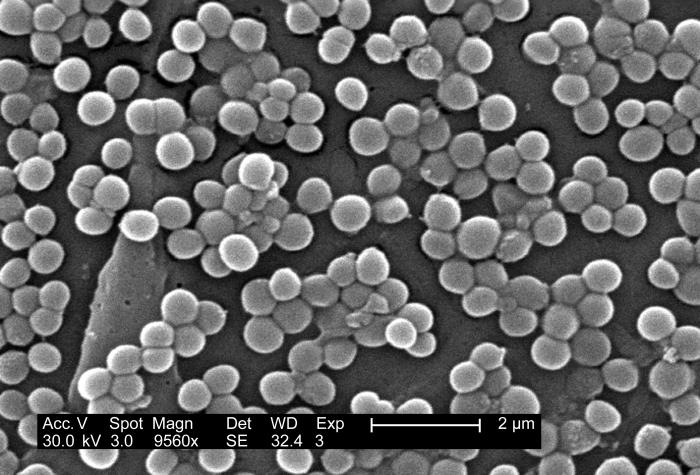
\includegraphics[scale=0.3]{saureus.jpg}
  %\caption{Imagen  de \textit{Staphylococcus aureus} obtenida con un microscopio electr\'onico de barrido (SEM). Tomado de \cite{HaneyCar2005PublicAureus}.}
  %\label{fig:sta}
%\end{center}
%\end{figure}

Desde el descubrimiento de \textit{Staphylococcus aureus} como causante de una infecci\'on a una herida en 1881 \cite{Orent2006AMagazine} se ha investigado su presencia en otras infecciones y se han utilizado antibi\'oticos como la penicilina, la meticilina y la vancomicina para controlar estas infecciones   \cite{HarpavatS.NissimS.LipppincottsMicrocards:MicrobiologyFlashCards2012.}. No obstante, \textit{Staphylococcus aureus} ha desarrollado resistencia a algunos de estos antibi\'oticos,  de ah\'{i} que surja la necesidad de buscar nuevos antibi\'oticos o incluso mol\'{e}culas con un mecanismo de acci\'{o}n diferente. Una posible familia de mol\'{e}culas que podr\'{i}an actuar como alternativas ser\'{i}an los p\'{e}ptidos antimicrobianos.\\

De acuerdo a Perez-Lopez et al. \cite{Perez-LopezVariationsProperties} y Nagendra et al.  \cite{Nagendra2011} se ha encontrado que la bacteria modula la composici\'{o}n de su membrana plasm\'{a}tica frente a cambios en el medio. Esta modulaci\'{o}n afecta las propiedades biof\'{i}sicas de su membrana, es decir propiedades fisicoqu\'{i}micas como la permeabilidad, la estructura y las propiedades mec\'{a}nicas. El cambio de estas propiedades es un factor que mejora la tolerancia de la bacteria a la acci\'{o}n de p\'{e}ptidos antimicrobiales. Debido a esto, las propiedades biof\'{i}sicas de la membrana se convierten en objeto de estudio y adem\'{a}s son determinantes en la b\'{u}squeda de nuevas mol\'{e}culas dirigidas a la membrana (mol\'{e}culas blanco) que combatan la bacteria. \\

Al ser \textit{Staphylococcus aureus}\footnote{\textit{Staphylococcus aureus} al ser una bacteria Gram positiva est\'{a} envuelta por una  membrana llamada bicapa lip\'{i}dica y recubierta de una pared externa de p\'{e}ptidoglicando. Las membranas se explican en la subsecci\'{o}n \ref{ss:mem}} una bacteria Gram positiva, consta de una membrana plasm\'{a}tica que es de inter\'{e}s en t\'{e}rminos de la generaci\'{o}n de nuevos antibi\'{o}ticos antimicrobiales debido a su rol como mediador del potencial electroqu\'{i}mico. Algunos estudios se han enfocado en c\'{o}mo la composici\'{o}n de la bicapa lip\'{i}dica interna afecta sus propiedades biof\'{i}sicas con base en cambios en la concentraci\'{o}n de ciertos l\'{i}pidos como la cardiolipina \cite{Hernandez-Villa1BiophysicalPeptides} y de carotenoides como la estafiloxantina \cite{MelendezDelgado2018StudyingBilayers}, \cite{Perez-LopezVariationsProperties}, \cite{Nagendra2011}. Recientemente, en nuestros grupos, se han estudiado computacionalmente y experimentalmente propiedades mec\'{a}nicas como la rigidez de la membrana, la orientaci\'{o}n de la estafiloxantina, el \'{a}rea por l\'{i}pido, la difusi\'{o}n y el par\'{a}metro de orden del deuterio de diferentes membranas modelo.\\

En los experimentos realizados por Perez-Lopez et al. \cite{Perez-LopezVariationsProperties} y Nagendra et al.  \cite{Nagendra2011} se ha mostrado que cambios en el contenido de carotenoides en las membranas, en diferentes etapas de crecimiento \textit{Staphylococcus aureus}, y en membranas modelo compuestas por algunos l\'{i}pidos mayoritarios de la bacteria, resultan en cambios en la rigidez. Se ha demostrado que este cambio en rigidez afecta la resistencia de la membrana a diferentes p\'{e}ptidos antimicrobiales. Sin embargo, es necesario mirar a nivel molecular la influencia local que tienen los carotenoides en la membrana para entender como la presencia de estas mol\'{e}culas puede influir en las propiedades mec\'{a}nicas. Debido a su resoluci\'{o}n, los experimentos realizados no permiten vislumbrar diferentes propiedades moleculares que puedan explicar este fen\'{o}meno. Alternativamente, las simulaciones de din\'{a}mica molecular (MD por sus siglas en ingl\'{e}s) si permiten hacer este acercamiento. La MD se ha convertido en una herramienta excelente para estudiar membranas biol\'{o}gicas \cite{Marrink2019ComputationalMembranes}. Este m\'{e}todo monitorea la evoluci\'{o}n espacio-temporal de sistemas biol\'{o}gicos a una escala at\'{o}mica y asi permite determinar informaci\'{o}n estructural (termo)din\'{a}mica y energ\'{e}tica de membranas, que complementa y expande las t\'{e}cnicas experimentales. 
Entre las propiedades que se pueden estudiar en detalle a trav\'{e}s de simulaciones est\'{a}n la ubicaci\'{o}n relativa de los carotenoides con respecto a los otros l\'{i}pidos, la orientaci\'{o}n y las interacciones que presenta exclusivamente el carotenoide estafiloxantina con los l\'{i}pidos vecinos. Estos detalles moleculares influyen en los cambios de la rigidez de la membrana de \textit{Staphylococcus aureus}.\\

Para estudiar la ubicaci\'{o}n, las interacciones con otros l\'{i}pidos, el \'{a}rea por l\'{i}pido,  de la estafiloxantina, en nuestro grupo se ha realizado un estudio computacional preeliminar mediante las simulaciones por din\'{a}mica molecular  implementadas en CHARMM \cite{MelendezDelgado2018StudyingBilayers}. Estas simulaciones requieren introducir ciertos par\'{a}metros relacionados con los campos de fuerza y con la geometr\'{i}a de la estafiloxantina, los cuales deben ser cuidadosamente seleccionados para que las simulaciones por din\'{a}mica molecular reflejen el comportamiento f\'{i}sico de la mol\'{e}cula.\\

En una aproximaci\'{o}n inicial, Mel\'{e}ndez et al. \cite{MelendezDelgado2018StudyingBilayers} utilizaron el protocolo implementado en CHARMM-GUI \cite{Sunhwan2008CHARMM-GUI:CHARMM} para determinar los par\'{a}metros de estafiloxantina. Algunos de los par\'{a}metros obtenidos a trav\'{e}s de este procedimiento para la estafiloxantina no se han optimizado completamente. El objetivo de la  presente propuesta es optimizar los par\'{a}metros generados por CHARMM-GUI para la estafiloxantina, para que luego puedan ser utilizados en simulaciones MD a la luz del trabajo previo realizado \cite{MelendezDelgado2018StudyingBilayers}. Adicionalmente, proponemos modelar la estafiloxantina utilizando un segundo campo de fuerzas (llamado AMBER). \'{e}ste modelamiento nos permitir\'{a} estudiar la din\'{a}mica de bicapas lip\'{i}dicas en presencia de estafiloxantina y confirmar que las observaciones que hagamos sean independientes del potencial de fuerzas utilizado.\\
\chapter{Cap\'{\i}tulo 1}
\subsection{La membrana Bacteriana y sus compuestos presentes}\label{ss:mem}
Seg\'{u}n el tipo de membrana que posean las bacterias, est\'{a}s pueden clasificarse en dos grandes clases: las bacterias Gram positivas y las bacterias Gram negativas. Las bacterias Gram positivas poseen una sola bicapa lip\'{i}dica envuelta en una capa compuesta por unos pol\'{i}meros de az\'{u}cares y amino\'{a}cidos llamados peptidoglicando (ver figura \ref{fig:mem}), mientras que las membranas de bacterias Gram negativa poseen dos bicapas lip\'{i}dicas. Ya que \textit{Staphylococcus aureus} es una bacteria Gram positiva se discutir\'{a} principalmente la composici\'{o}n de la membrana de las bacterias Gram Positivas.\\

\begin{figure}[h]
\begin{center}
  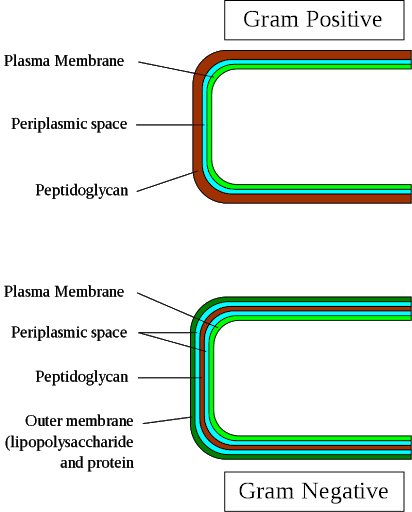
\includegraphics[scale=0.3]{Kap2/grampos1.png}
    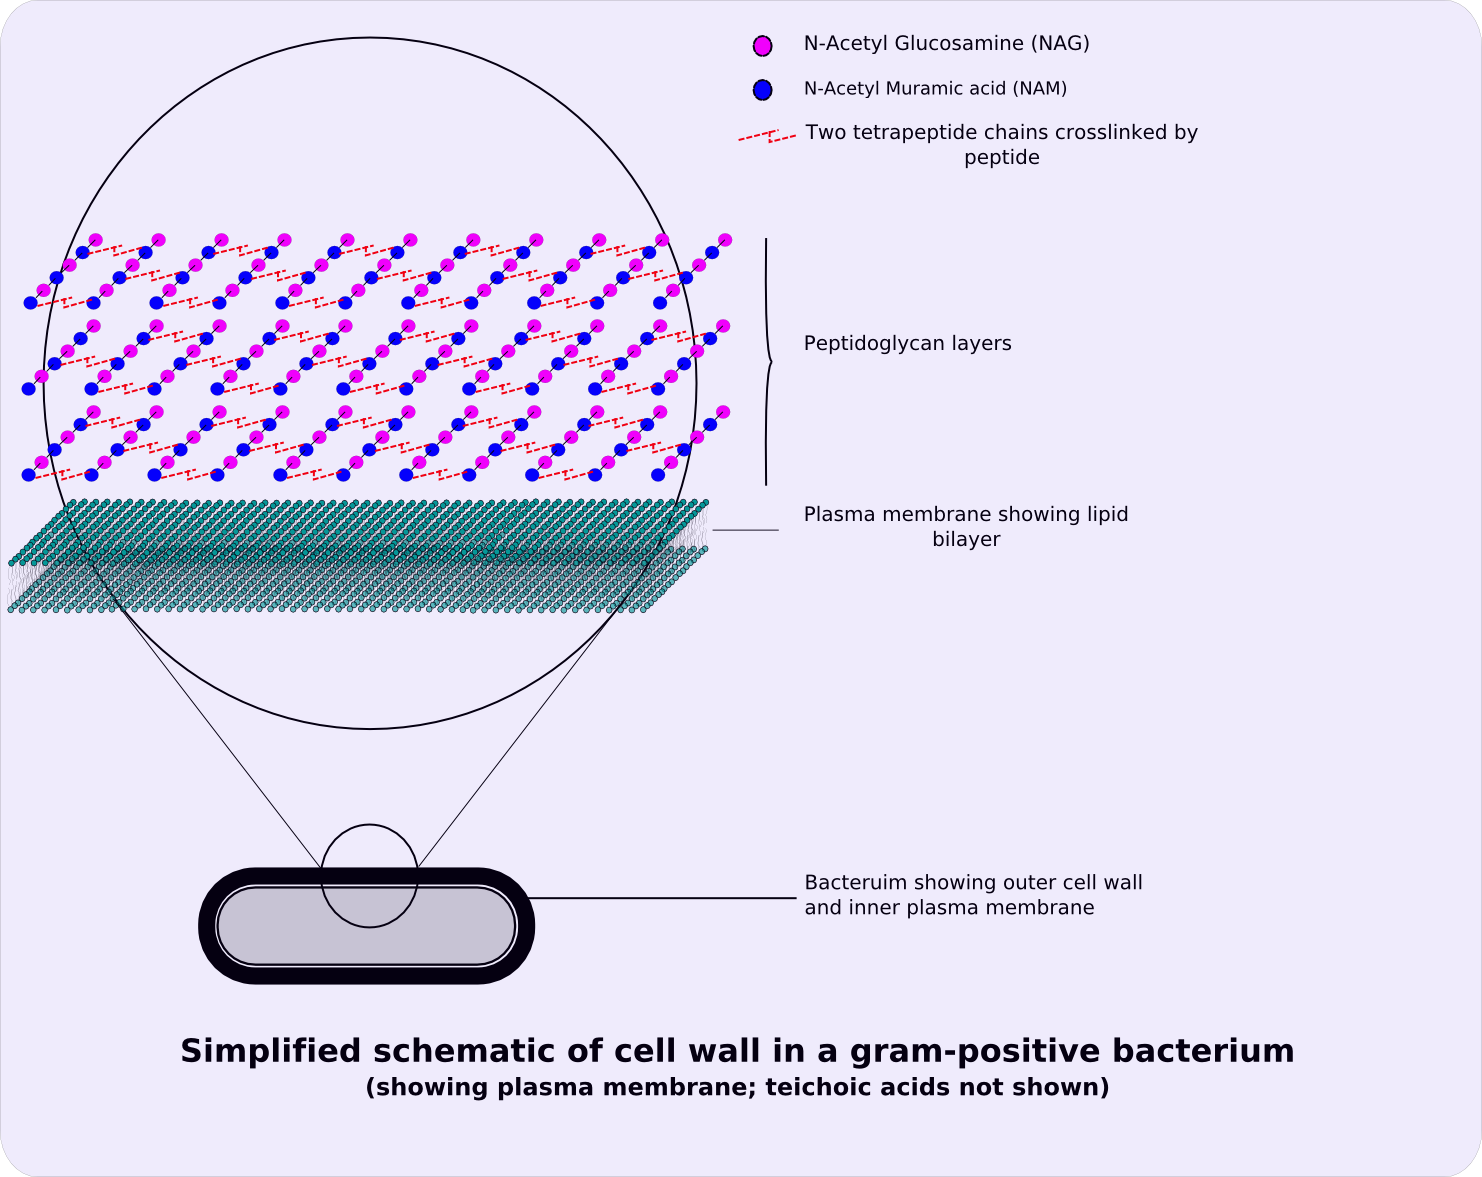
\includegraphics[scale=0.15]{Kap2/grampos2.png}
  \caption{Imagen  de la membrana de una bacteria Gram positiva. Tomado de \cite{Nelson2011}.}
  \label{fig:mem}
\end{center}
\end{figure}
La bicapa lip\'{i}dica es una membrana presente en todos las c\'{e}lulas la cual est\'{a} compuesta mayoritariamente por l\'{i}pidos. Los l\'{i}pidos se acomodan de tal manera que el espesor de la membrana sea de dos l\'{i}pidos de grosor. En su mayor\'{i}a, con excepciones como los esteroles, los l\'{i}pidos est\'{a}n compuestos por una o varias cadenas de \'{a}cidos grasos no polares (cadenas hidrocarbonadas con carboxilo) unidas a diferentes sustituyentes polares los cuales pueden presentar carga o no a pH fisiol\'{o}gico. De acuerdo a los sustituyentes y al tipo de \'{a}cidos grasos, cada l\'{i}pido presenta propiedades fisicoqu\'{i}micas espec\'{i}ficas como la carga total, la polaridad, y el largo que lo distinguen a nivel biof\'{i}sico con los otros l\'{i}pidos. Los l\'{i}pidos forman bicapas debido a la presencia del agua ya que al ser mol\'{e}culas anfip\'{a}ticas (combinando motivos polares y apolares) se orientan con respecto a esta. La parte hidrof\'{i}lica del l\'{i}pido interact\'{u}a con el agua mientras que la parte hidrof\'{o}bica no interact\'{u}a con esta, lo que induce reorientaci\'{o}n y agregaci\'{o}n de los l\'{i}pidos. Estas interacciones hacen que sea m\'{a}s estable encontrar los l\'{i}pidos inmersos en el agua formando agregados sin mezclarse con el agua. La interacci\'on lateral entre estas mol\'eculas se da a trav\'es de fuerzas no covalentes lo que le confiere propiedades de cristal l\'iquido caracterizado por la capacidad de presentar transiciones de fase s\'olido-l\'iquido y difusi\'{o}n lateral. \\

La bicapa lip\'{i}dica de \textit{Staphylococcus aureus} esta compuesta principalmente por fosfatidilgliceroles (PG), cardiolipina (CL), lifosfoglicandos (LPG) y glicopeptidol\'{i}pidos (GPL) \cite{Sohlenkamp2015BacterialPathways}. En la figura \ref{fig:DMPG} se muestra la f\'{o}rmula estructural del Dimiristoilfosphatidilglicerol (DMPG), el cual es un l\'{i}pido con el fosfatidilglicerol unido a dos miristoil (provenientes del \'{a}cido mir\'{i}stico). 
\\

\begin{figure}[h]
\begin{center}
    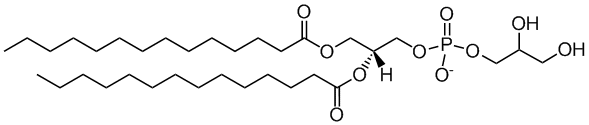
\includegraphics[scale=0.4]{Kap2/DMPG.png}
  \caption{F\'{o}rmula estructural del Dimiristoilfosphatidilglicerol (DMPG). Tomada de \cite{CHEMDRUGDMPGDimyristoylphosphatidylglycerol}.}
  \label{fig:DMPG}
\end{center}
\end{figure}
Las membranas lip\'{i}dicas adem\'{a}s de tener l\'{i}pidos contienen otros tipos de biomol\'{e}culas como los carotenoides, las prote\'{i}nas y los glicol\'{i}pidos que tienen relevancia fisiol\'{o}gica en la c\'{e}lula. Los carotenoides en particular pigmentan las c\'{e}lulas. En el caso de \textit{Staphylococcus aureus} se ha descubierto que los carotenoides juegan un papel importante en la integridad de la membrana celular y protegen a la bacteria frente a estr\'{e}s oxidativo \cite{Nagendra2011}. La protecci\'{o}n de los carotenoides en la membrana se ve reflejada por un aumento de su rigidez, de forma similar al papel que juega el colesterol en la membrana eucari\'{o}tica. \\

Uno de los carotenoides m\'{a}s relevantes en \textit{Staphylococcus aureus} es la estafiloxantina la cual le da el nombre a la bacteria ya que le da un color a\'{u}reo. La estafiloxantina es un  triterpeno carotenoide que posee dos cadenas hidrocarbonadas. Una de ellas es un \'{a}cido graso parecido a otros acidos grasos de la membrana, caracterizado por ser saturado y con presencia de ramificaciones metiles. El otro es un \'{a}cido graso diaponeurosporenoico, que presenta insaturaciones conjugadas tipo trans y ramificaciones.  Las dos cadenas est\'{a}n unidas a un mol\'{e}cula de glucosa mediante enlaces tipo \'{e}ster, ver figura \ref{fig:stx}. Debido a los enlaces dobles conjugados de la cadena diaponeurosporenoica, esta es r\'{i}gida, ya que estos enlaces dificultan rotaciones intramoleculares. Esta rigidez se convierte en un factor que aumenta el empaquetado de la bicapa l\'{i}p\'{i}dica, ya que disminuye la distancia entre l\'{i}pidos vecinos \cite{Heimburg}.\\

\begin{figure}[h]
\begin{center}
  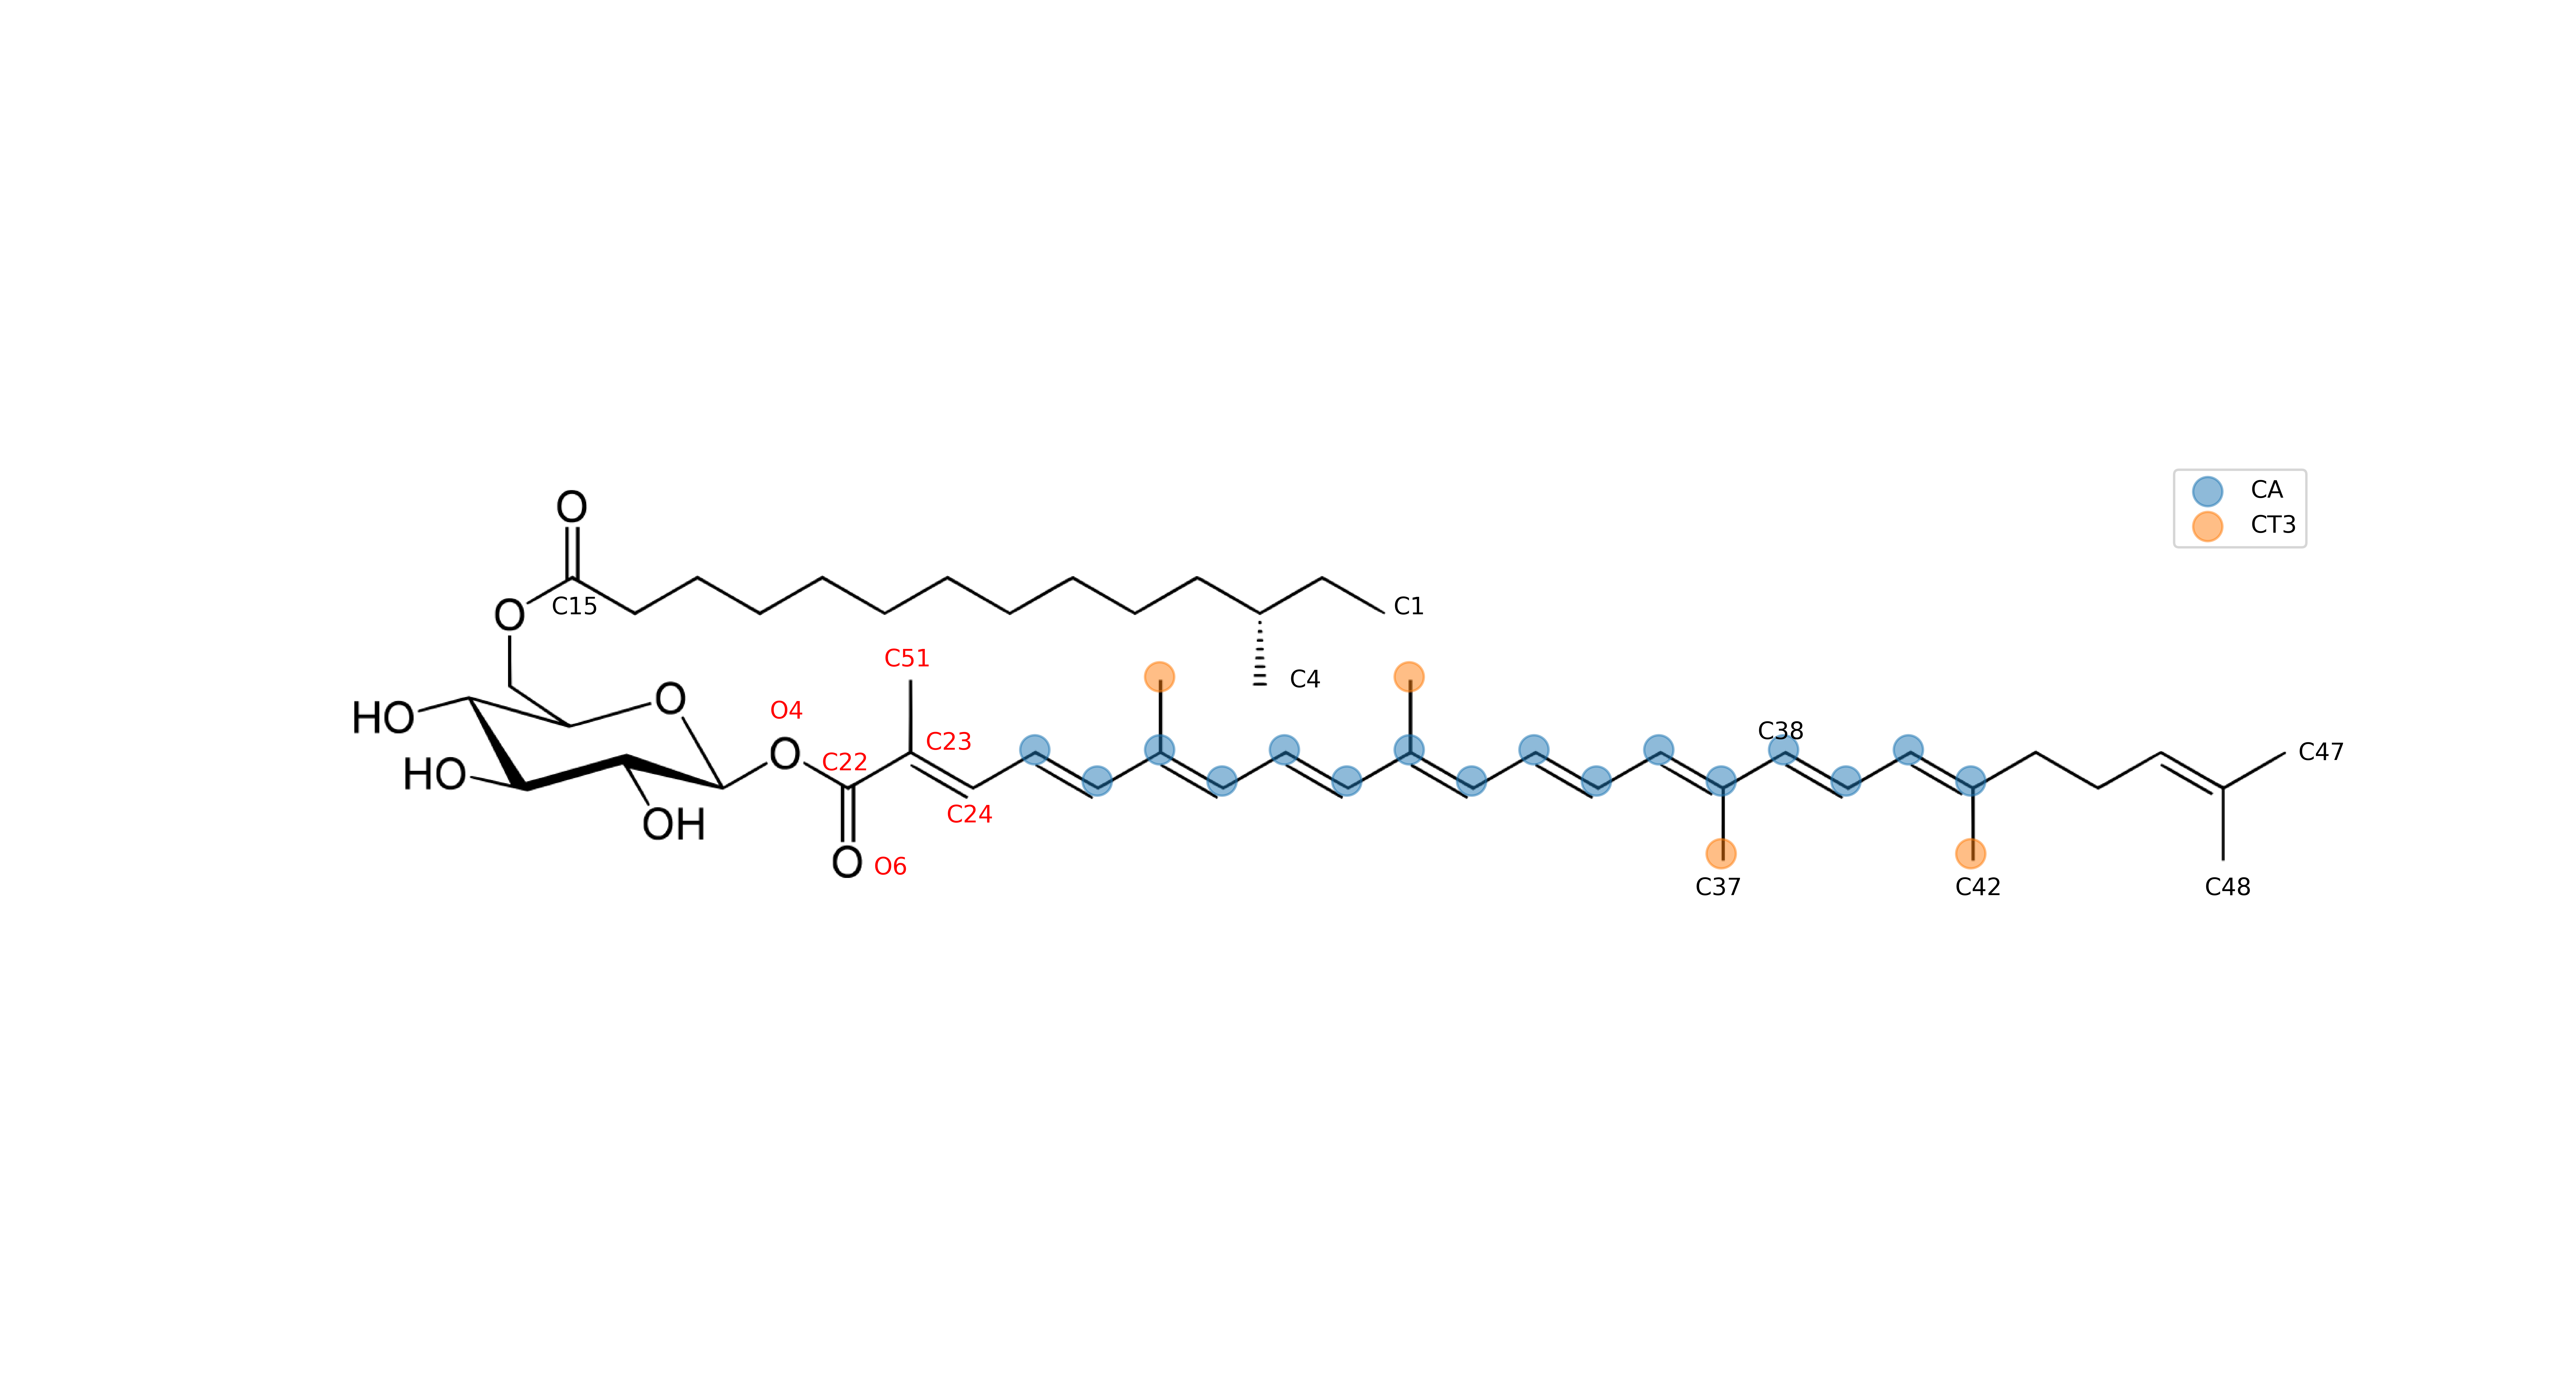
\includegraphics[scale=0.4]{Kap2/stx_problems.png}
  \caption{F\'{o}rmula estructural de la estafiloxantina. Tomada de \cite{MelendezDelgado2018StudyingBilayers}.}
  \label{fig:stx}
\end{center}
\end{figure}
 Adem\'{a}s, estas insaturaciones conjugadas le dan propiedades antioxidantes que protegen a la bacteria frente al estr\'{e}s oxidativo del medio, al poder incorporar especies reactivas oxidativas \cite{Nelson2011}.
\subsection{Resistencia a tratamientos antibi\'{o}ticos de \textit{Staphylococcus aureus}}\label{ss:anti}
Desde el descubrimiento de la penicilina, infecciones de \textit{Staphylococcus aureus} han sido tratadas con este antibi\'{o}tico. Sin embargo, a mediados del siglo XX \textit{Staphylococcus aureus} comenz\'{o} a presentar resistencia a esta familia de antibi\'{o}ticos $\beta$-lact\'{a}micos, incluida la meticilina. Posteriormente se han aplicado otros antibi\'{o}ticos como la vancomicina, pero tambi\'{e}n se ha ido generando  resistencia a estos otros antibi\'{o}ticos.  De la resistencia a antibi\'{o}ticos surge la necesidad de buscar nuevos medicamentos que combatan \textit{S. aureus}.\\

Un p\'eptido antimicrobiano es  un olig\'omero de amino\'acidos, de alrededor de 20 aminoacidos de largo, que hace parte de la respuesta inmune de un amplio espectro de especies, y que son faciles de sintetizar en el laboratorio. Los p\'{e}ptidos antimicrobianos se clasifican seg\'{u}n la estructura secundaria que tienen: $\alpha$ h\'elices, $\beta$ plegados.   Los p\'eptidos antimicrobianos interact\'uan con la membrana de la bacteria produciendo orificios que causan p\'erdida de contenido, p\'{e}rdida del potencial electroqu\'{i}mico y muerte celular.\\

Los p\'{e}ptidos antimicrobiales forman estructuras anfip\'{a}ticas que inducen su adhesi\'{o}n a la membrana. Al aumentar su concentraci\'{o}n superficial, se induce una inserci\'{o}n de estos p\'{e}ptidos, atravesando la membrana y generando poros. Son de inter\'{e}s los p\'{e}ptidos antimicrobiales cati\'{o}nicos ya que la membrana de \textit{Staphylococcus aureus} es ani\'{o}nica y estos p\'{e}ptidos tienen una preferencia para adherirse a estas membranas. La formaci\'{o}n de poros es un proceso mec\'{a}nico que requiere la deformaci\'{o}n de la membrana para suceder. Al incrementar la rigidez de la membrana, se dificulta la inserci\'{o}n del p\'{e}ptido generando resitencia \cite{Perez-LopezVariationsProperties}, \cite{Nagendra2011}. Por este motivo se vuelve relevante estudiar como la composici\'{o}n de la membrana, en particular la presencia de stafiloxantina, modula la rigidez de la membrana.

\chapter{Cap\'{\i}tulo 2:Simulaciones de Membranas}
\section{Din\'{a}mica Molecular y Campos de Fuerza}\label{ss:md} 
Un paradigma central en la biolog\'{i}a es la existencia de un v\'{i}nculo entre la secuencia, la estructura, la din\'{a}mica y la funci\'{o}n de una biomol\'{e}cula, enti\'{e}ndase esta \'{u}ltima como cualquier mol\'{e}cula con un rol biol\'{o}gico \cite{Cui2006}. No \'{u}nicamente la secuencia de amino\'{a}cidos o secuencia de nucle\'{o}ticos, sino tambi\'{e}n la estructura y a la din\'{a}mica son determinantes en la funci\'{o}n de cualquier biomol\'{e}cula. En el caso de las membranas biol\'{o}gicas, la complejidad aumenta, ya que a las prote\'{i}nas de membrana, que se encargan de diversas funciones fisiol\'{o}gicas para las c\'{e}lulas y sus organelos, se suma una rica composici\'{o}n de l\'{i}pidos. Los l\'{i}pidos no son entes pasivos que proveen un medio bidimensional para las prote\'{i}nas de membrana. Por el contrario, ellos afectan tanto las propiedades bioqu\'{i}micas como las propiedades f\'{i}sicas, como la movilidad y la rigidez de las membranas y as\'{i} en \'{u}ltimas influir en su funci\'{o}n.\\

Un m\'{e}todo poderoso para estudiar la din\'{a}mica de biomol\'{e}culas, y en particular las membranas biol\'{o}gicas, es el de las simulaciones por din\'{a}mica molecular (MD por sus siglas en ingl\'{e}s).\\

En la din\'{a}mica molecular se resuelven num\'{e}ricamente las ecuaciones de movimiento de Newton para cada una de las part\'{i}culas que constituyen el sistema, por ejemplo a nivel de \'{a}tomos (alta resoluci\'{o}n espacial) o grupos de atomos (menor resoluci\'{o}n espacial), de donde se obtiene la trayectoria en funci\'{o}n del tiempo de cada part\'{i}cula. Una vez obtenida la trayectoria se pueden analizar las propiedades del sistema en estudio, a partir las velocidades, posiciones y energ\'{i}as de interacci\'{o}n de todo el sistema, registradas durante la simulaci\'{o}n.\\

Las ecuaciones de movimiento de Newton para un conjunto de $N$ part\'{i}culas (3N coordenadas) est\'{a}n restringidas a una funci\'{o}n de energ\'{i}a potencial, denominada $V(\vec{r})$, dependiente solo de la distancia entre part\'{i}culas y afectando las fuerzas y torques de interacci\'{o}n. Estas ecuaciones tienen la forma \cite{Goldstein2001}:

\begin{equation}\label{eq:1}
m_i\frac{\mathrm{d}^2\vec{r_i}}{\mathrm{d}t^2}=-\vec{\nabla_i}V(\vec{r}_1,...,\vec{r}_N) \text{\hspace{30pt}}i=1,2,...,N,
\end{equation}
donde $m_i$ es la masa de la $i$-\'{e}sima part\'{i}cula, $\vec{r_i}$ es su posici\'{o}n y el gradiente $ \vec{\nabla_i}$ se calcula sobre las coordenadas de posici\'{o}n de la $i$-\'{e}sima part\'{i}cula.\\

Para resolver las ecuaciones de movimiento es necesario conocer la fuerza aplicada al sistema en cada instante de tiempo, esta se halla a partir de la energ\'{i}a potencial sobre las part\'{i}culas. En la secci\'{o}n de Campos de fuerza se detalla la naturaleza de estos potenciales.
\section{Campos de Fuerza}
Un campo de fuerza (o \textit{force field} e ingl\'{e}s) es un conjunto de t\'{e}rminos emp\'{i}ricos que modelan la interacci\'{o}n entre mol\'{e}culas. El prop\'{o}sito de estos es poder representar la energ\'{i}a potencial de un conjunto de part\'{i}culas interactuantes a trav\'{e}s de funciones aritm\'{e}ticas simples, que puedan ser evaluadas num\'{e}ricamente de manera eficiente a trav\'{e}s del computador \cite{Kukol2014MolecularEdition}. Algunos de los campos de fuerza m\'{a}s utilizados para biomol\'{e}culas son AMBER, CHARMM, GROMOS y OPLS-AA. Todos estos campos de fuerza tienen en com\'{u}n la separaci\'{o}n de la energ\'{i}a potencial en dos t\'{e}rminos: interacciones enlazantes e interacciones no enlazantes. En forma de ecuaci\'{o}n un campo de fuerza t\'{i}picamente contiene los siguientes t\'{e}rminos:
\begin{equation}\label{eq:5}
    V=V_{\text{enlazante}}+V_{\text{no enlazante}}
\end{equation}
Cada uno de estos est\'{a} a su vez compuesto por los siguientes t\'{e}rminos:
\begin{itemize}
\item Interacciones enlazantes: $V_{cov}$, que tienen en cuenta los enlaces covalentes entre \'{a}tomos; $V_{ang}$, vibraciones angulares entre triadas de \'{a}tomos y $V_{tor}$, movimientos de torsi\'{o}n entre grupos de cuatro \'{a}tomos conectados por dos enlaces covalentes:
\begin{eqnarray}\label{eq:6}
V_{cov}(r)&=&\sum_{enlaces}k_r\left(r-r_0\right)^2\\
V_{ang}(r)&=&\sum_{val}k_\theta\left(\theta-\theta_{0}\right)^2\\
V_{tor}(r)&=&\sum_{dihedros}\sum_{n}\frac{V_n}{2}\left[1+\cos(n\phi-\gamma)\right]
\end{eqnarray}
\item Interacciones no enlazantes: que se componen de interacciones de corto alcance de Van der Waals, modeladas a trav\'{e}s de un potencial de Lennard Jones, $V_{LJ}$ e interacciones eletrost\'{a}ticas descritas por medio del potencial de Coulomb, $V_{Coul}$.
\begin{eqnarray}\label{eq:7}
V_{LJ}(r)&=&\sum_{j=1}^{N+1}\sum_{i=j+1}^N f_{ij}\left\{\epsilon_{ij}\left[\left(\frac{r_{0ij}}{r_{ij}}\right)^{12}-2\left(\frac{r_{0ij}}{r_{ij}}\right)^6\right]\right\}\\
V_{Coul}(r)&=&\sum_{j=1}^{N-1}\sum_{i=j+1}^{N}\frac{q_iq_j}{4\pi\epsilon_0\epsilon_R r_{ij}}
\end{eqnarray}
\end{itemize}
Las constantes $k_r,k_\theta,f_{ij},\epsilon_{ij},r_{0ij},q_{i},q_{j}$ son las constantes emp\'{i}ricas que definen el campo de fuerzas. Estas constantes se determinan de distintas maneras , por ejemplo a trav\'{e}s de c\'{a}lculos de mec\'{a}nica cu\'{a}ntica o por optimizacionres para reproducir propiedades termodin\'{a}micas de los sistemas en cuesti\'{o}n como energ\'{i}as de solvataci\'{o}n y funciones de partici\'{o}n.

Una de las diferencias entre los programas est\'{a} en el tratamiento de los \'{a}ngulos dihedros impropios, es decir de los involucrados en la quiralidad de las mol\'{e}culas. Por ejemplo, CHARMM Y GROMOS agregan a las interacciones enlazantes un potencial arm\'{o}nico entre los \'{a}tomos terminales del dihedro (en A-B-C-D ser\'{i}an A y C) denomindado de Urey-Bradley con la forma:
\begin{equation}\label{eq:8}
    V_{\mathrm{UB}}=\sum_{\mathrm{Urey-Bradley}} K_{\mathrm{UB}}(b^{A-C}-b^{A-C,0})^2
\end{equation}
En AMBER y OPLS-AA esta interacci\'{o}n es incluida en el t\'{e}rmino del potencial de torsiones.\\

En cuanto a los par\'{a}metros de los t\'{e}rminos enlazantes tanto AMBER como CHARMM calculan las constantes de los t\'{e}rminos no enlazantes/entre pares de \'{a}tomos $i$,$j$ como:
\begin{equation}\label{eq:9}
   \epsilon_{ij}=\sqrt{\epsilon_{i}\epsilon_{j}}
\end{equation}
\begin{equation}\label{eq:10}
   r_{0ij}=\frac{1}{2}\left(r_i+r_j\right)
\end{equation}
\section{Soluci\'{o}n de las ecuaciones de Movimiento}
Debido al tama\~no de los sistemas biol\'{o}gicos a considerar, en el caso de estafiloxantina embebida en una bicapa con 128 l\'{i}pidos de DMPG (O DPPG) del orden de 15000 \'{a}tomos \cite{MelendezDelgado2018StudyingBilayers}, las ecuaciones de movimiento \eqref{eq:1} deben resolverse num\'{e}ricamente. Para resolverlas se usan algoritmos como el de Verlet, el de ``\textit{leapfrog}'', el de velocidad de Verlet o el de Beeman \cite{Mazur1997CommonRevisited}.\\
En el algoritmo de Verlet se hace una aproximaci\'{o}n en series de Taylor a segundo orden de las posiciones hacia adelante $\vec{r}_{i}(t_{n+1})$ y hacia atr\'{a}s $\vec{r}_{i}(t_{n-1})$, ver \cite{MelendezDelgado2018StudyingBilayers},\cite{Mazur1997CommonRevisited}; que al restarlas da la siguiente soluci\'{o}n iterada:
\begin{equation}\label{eq:2}
t_{n}=n\Delta t
\end{equation}
\begin{equation}\label{eq:3}
\vec{r}_{(i,t_{n+1})}=2\vec{r}_{(i,t_{n})}-\vec{r}_{(i,t_{n-1})}+\vec{a}_{(i,t_{n})}(\Delta t)^2
\end{equation}
\begin{equation}\label{eq:4}
\vec{v}_{(i,t_{n})}=\frac{\vec{r}_{(i,t_{n+1})}-\vec{r}_{(i,t_{n-1})}}{2\Delta t}
\end{equation}
Donde la ecuaci\'{o}n \eqref{eq:4} para la velocidad es una expresi\'{o}n de diferencias finitas y se obtuvo mediante el promedio entre $v_{(i,tn+\Delta t/2)}$ y $v_{(i,tn-\Delta t/2)}$.
Obs\'{e}rvese que las ecuaciones \eqref{eq:3} y \eqref{eq:4} solo dependen de las coordenadas anteriores y no de las velocidades. Luego, solo es necesario usar la ecuaci\'{o}n \eqref{eq:3} para encontrar la trayectoria de la part\'{i}cula.\\

En el algoritmo de ``leapfrog" se resuelven las ecuaciones de movimiento \eqref{eq:1} hallando las posiciones de las part\'{i}culas para los tiempos $t_1,t_2=t_1+\Delta t,...,t_n=t_{1}+n\Delta t$, mientras que las velocidades de las part\'{i}culas se hallan para los tiempos $t_1-\Delta t/2,t_2=t_1+\Delta t/2,...,t_n=t_{1}+(n-1/2)\Delta t$, ver \cite{Mazur1997CommonRevisited}.  Este algoritmo tiene la forma:
\begin{equation}\label{eq:5}
\vec{v}{(i,t_{n+1/2})}=\vec{v}{(i,t_{n-1/2})}+\vec{a}{(i,t_{n})}\Delta t,
\end{equation}
\begin{equation}\label{eq:6}
\vec{r}{(i,t_{n+1})}=\vec{r}{(i,t_{n-1})}+\vec{v}{(i,t_{n+1/2})}\Delta t.
\end{equation}
Como se han aproximado las ecuaciones para la velocidad y para la aceleraci\'{o}n a una l\'{i}nea recta, entonces el valor medio de las velocidad entre los tiempos $t_{n-1/2}$ y $t_{n+1/2}$ es:
\begin{equation}\label{eq:7}
\vec{r}{(i,t_{n+1})}=\vec{r}{(i,t_{n-1})}+\vec{v}{(i,t_{n+1/2})}\Delta t.
\end{equation}
Utilizando las ecuaciones \eqref{eq:5}, \eqref{eq:6} y \eqref{eq:7} se obtiene otra forma de escribir el algoritmo de leapfrog:
\begin{eqnarray}
  x_{i+1} &= x_i + v_i\, \Delta t + \tfrac{1}{2}\,a_i\, \Delta t^{\,2}, \\
  v_{i+1} &= v_i + \tfrac{1}{2}(a_i + a_{i+1})\,\Delta t.
\end{eqnarray}

Por otro lado, las condiciones iniciales para resolver los algoritmos pueden ser obtenidas por m\'{e}todos experimentales como la cristalograf\'{i}a de rayos-X, resonancia magn\'{e}tica nuclear o microscop\'{i}a electr\'{o}nica criog\'{e}nica (m\'{a}s com\'{u}n en prote\'{i}nas y \'{a}cidos nucl\'{e}icos) o computacionalmente para sistemas de muchas mol\'{e}culas, realizando un autoensamblaje y minimizando la energ\'{i}a del ensamblaje. Las velocidades iniciales se generan de manera aleatoria a partir de la distribuci\'{o}n Maxwell-Boltzmann para la energ\'{i}a cin\'{e}tica a una temperatura $T$ dada.\\
%\vec{v}_{i}(t_{n}+\Delta t/2)=\vec{v}_i(t_{n}-\Delta t/2)+\frac{\Delta t}{m_i}\vec{F}_{i}(t_{n})
\section{Simulaciones en Membranas}\label{ss:smem}
\section{Trabajo Preliminar}\label{ss:pre}
\subsection{Estudio del Rol de Estafiloxantina en la modulaci\'{o}n de par\'{a}metros estructurales de bicapas lip\'{i}dicas compuestas por DMPG y DPPG  \cite{MelendezDelgado2018StudyingBilayers}}
Para estudiar el rol de la estafiloxantina en bicapas lip\'{i}dicas compuestas por dimiristoil fosfatidilglicerol (DMPG) y dipalmitoil fosfatidilglicerol (DPPG) Mel\'{e}ndez et al. \cite{MelendezDelgado2018StudyingBilayers} realizaron simulaciones por din\'{a}mica molecular para 4 sistemas con las siguientes composiciones: DMPG, DMPG$+$estafiloxantina, DPPG y DPPG$+$estafiloxantina. De los resultados obtenidos de estas simulaciones se obtuvieron par\'{a}metros que dan cuenta del efecto de la estafiloxantina en los l\'{i}pidos circundantes a nivel global y local, as\'{i} como su orientaci\'{o}n dentro de la membrana. Estos par\'{a}metros incluyen el par\'{a}metro de orden del Deuterio $S_{CD}$, el espesor de la membrana, el coeficiente lateral de difusi\'{o}n y el \'{a}rea por l\'{i}pido. \\

Estas simulaciones revelaron que la estafiloxantina adopta dos orientaciones diferentes respecto a la membrana. La estafiloxantina se encontr\'{o} mayoritariamente alrededor de los 100\textdegree para el sistema   DMPG+estafiloxantina. Para el sistema  DPPG+estafiloxantina muestre\'{o} dos \'{a}ngulos preferenciales,  uno m\'{a}s probable alrededor de 100\textdegree y otro un poco menos probable, alrededor de 135\textdegree. Los \'{a}ngulos menores a 120\textdegree representan una orientaci\'{o}n horizontal de la estafiloxantina y los mayores a 120\textdegree  una orientaci\'{o}n vertical respecto al plano normal de la membrana.\\

La orientaci\'{o}n horizontal es un resultado inesperado, pues esta es una conformaci\'{o}n inusual para l\'{i}pidos. Esto nos llev\'{o} a pensar que algunos de los par\'{a}metros del campo de fuerzas de la estafiloxantina no estaban bien definidos. En efecto se encontr\'{o} que los par\'{a}metros de torsi\'{o}n, obtenidos a trav\'{e}s del servidor CHARMM-GUI para la cadena de enlaces dobles conjugados en la estafiloxantina, no son los m\'{a}s adecuados, debido a la inusual estructura del \'{a}cido daponourosporen\'{o}ico. Como alternativa se utilizaron los par\'{a}metros de torsi\'{o}n de grupos benceno, que tambi\'{e}n presentan insaturaciones conjugadas, para corregir los par\'{a}metros de la cadena diaponeurosporenoica. El uso de los par\'{a}metros de torsi\'{o}n del benceno permiti\'{o} que la cadena diaponeurosporenoica adoptara una estructura plana, esperada debido a la presencia de los enlaces dobles conjugados. Sin embargo, una validaci\'{o}n rigurosa de estos par\'{a}metros no ha sido realizada. Adicionalmente, los \'{a}ngulos de torsi\'{o}n entre los carbonos pr\'{o}ximos al grupo \'{e}ster (ver figura \ref{fig:stx}) reportaron una baja puntuaci\'{o}n durante la parametrizaci\'{o}n por CHARMM-GUI, debido a la presencia del grupo carboxilo que induce una redistribuci\'{o}n de la densidad electr\'{o}nica. Es necesario corregir los parametros tomando esto en cuenta. Adicionalmente, para descartar posibles artefactos introducidos por uno u otro campo de fuerzas en la orientaci\'{o}n preferente de estafiloxantina, se hace indispensable parametrizar esta mol\'{e}cula con otro conjunto de par\'{a}metros, por ejemplo AMBER.

\chapter{Cap\'{\i}tulo 3: Metodolog\'{i}a}
\section{Reproducci\'{o}n de las simulaciones realizadas por Mel\'{e}ndez et al. \cite{MelendezDelgado2018StudyingBilayers}}
\section{Realizaci\'{o}n de las simulaciones por din\'{a}mica molecular de estafiloxantina embebida en membranas de DMPG y DPPG colocando los par\'{a}metros obtenidos por optimizaciones QM}
\section{Realizaci\'{o}n de simulaciones de membranas de DMPG y DPPG con una concentraci\'{o}n de estafiloxantina al 15\% y estudio de sus propiedades}
\section{An\'{a}lisis de las Simulaciones}
\begin{enumerate}
\item \textbf{Reproducir las simulaciones por din\'{a}mica molecular de estafiloxantina en DMPG y DPPG realizadas  por Mel\'{e}ndez et al. \cite{MelendezDelgado2018StudyingBilayers}, utilizando los par\'{a}metros no optimizados de la cadena diaponeurosporenoica.}\label{item:1}\\

\textbf{Ensamblaje}\\
Se ensamblar\'{a}n las bicapas lip\'{i}dicas DMPG y DPPG mediante la herramienta de ensamblaje de CHARMM-GUI \cite{Sunhwan2008CHARMM-GUI:CHARMM}, insertando 64 l\'{i}pidos por monocapa. Adicionalmente, a cada sistema se le agregar\'{a}n 45 mol\'{e}culas de agua por l\'{i}pido,  un ion de \ce{Na^+} por l\'{i}pido  para contrarrestar la carga negativa y 0.15M de \ce{NaCl} para reproducir la condiciones fisiol\'{o}gicas de sal.\\
Dentro de esta membrana se insertar\'{a} posteriormente una mol\'{e}cula de estafiloxantina. Partiendo del archivo SMILES tomado de \cite{NationalCenterforBiotechnologyInformationPubChemCID=24892781} y utilizando tambi\'{e}n CHARMM-GUI se obtendr\'{a}n la estructura tridimensional y el campo de fuerzas de todo el sistema. Una vez finalizado este procedimiento se cambiar\'{a}n los t\'{e}rminos de los \'{a}ngulos dihedros  de la cadena diaponeurosporenoica por aquellos asociados a anillos arom\'{a}ticos, los cuales son mas representativos de un sistema deslocalizado de enlaces dobles conjugados parecido al que presenta la cadena diaponeurosporenoica.\\
\textbf{Minimizaci\'{o}n de la Energ\'{i}a}\\
Para remover sobrelapamiento entre \'{a}tomos durante el proceso de ensamblaje, que pueda causar inestabilidades durante las simulaciones de din\'{a}mica molecular, se realizar\'{a} una minimizaci\'{o}n de la energ\'{i}a, por 5000 pasos, usando el m\'{e}todo de gradiente decreciente. Est\'{a} simulaci\'{o}n se realizar\'{a} con el paquete de simulaci\'{o}n principal GROMACS \cite{AbrahamGROMACS2019}.\\

\textbf{Relajaci\'{o}n}\\
Las coordenadas obtenidas a partir de la minimizaci\'{o}n de la energ\'{i}a se relajar\'{a}n en 6 simulaciones de din\'{a}mica molecular sucesivas, de 25ps cada una, integrando las ecuaciones de movimiento a pasos discretos de tiempo de 1fs. Este valor es 10 veces menor al per\'{i}odo asociado a la frecuencias de vibraci\'{o}n m\'{a}s alta encontrada para este sistema, correspondiente a fluctuaciones en las posiciones en los \'{a}tomos de hidr\'{o}geno. Durante cada una de las equilibraciones se impondr\'{a}n restricciones en las posiciones y en los \'{a}ngulos dihedros de un \'{a}tomo en la cabeza de cada l\'{i}pido, con el fin de que estos no se desv\'{i}en significativamente de sus posiciones iniciales y que las cadenas lip\'{i}dicas no adopten orientaciones artificiales. Estas restricciones se ir\'{a}n removiendo gradualmente durante las 6 simulaciones de relajaci\'{o}n.\\

\textbf{Simulaci\'{o}n}\\
Se impondr\'{a}n condiciones de frontera peri\'{o}dicas en una caja ortorr\'{o}mbica. El sistema se mantendr\'{a} a una presi\'{o}n de 1bar y a temperatura de 323K constantes (condiciones termodin\'{a}micas NPT) acopl\'{a}ndolo a una barostato de Parinello-Rahman \cite{Parrinello1981PolymorphicMethod} y aun termostato de Nose-Hoover. Las interacciones no enlazantes de corto alcance se modelar\'{a}n mediante un potencial de Lennard-Jones (ecuaci\'{o}n \eqref{eq:7}). EL potencial de Coulomb (ecuaci\'{o}n 7) se calcular\'{a} por el medio del m\'{e}todo de \textit{Particle Mesh Ewald (PME)}, apropiado para sistemas peri\'{o}dicos \cite{Darden1993ParticleSystems}. Los enlaces relacionados con los \'{a}tomos de hidr\'{o}geno  se restringir\'{a}n a trav\'{e}s de ligaduras utilizando el algoritmo de LINCS \cite{Hess1997LINCS:Simulations} y para el caso del agua tambi\'{e}n el \'{a}ngulo entre los dos hidr\'{o}genos tambi\'{e}n el \'{a}ngulo entre los dos hidr\'{o}genos empleando el algoritmo SETTLE \cite{Miyamoto1992Settle:Models}. Estas restricciones permitir\'{a}n aumentar el paso de tiempo de integraci\'{o}n a 2fs. Para cada uno de los sistemas considerados se realizar\'{a} una simulaci\'{o}n de $1\mu$s.\\
%%%%%%%%%%%%%%%%%%%%%%%%%%%%%%%%%%%%%%%%%%%%%%%%%%%%%%%%%%%%%%%%%%%%%%%
\item \textbf{Optimizar los par\'{a}metros relacionados  con los \'{a}ngulos dihedros de la cadena diaponeurosporenoica pr\'{o}ximos al enlace \'{e}ster. Posteriormente, realizar simulaciones por din\'{a}mica molecular de estafiloxantina embebida en membranas de DMPG y DPPG.}\label{item:2}\\

Los \'{a}ngulos dihedros de la cadena diaponeurosporenoica pr\'{o}ximos al enlace \'{e}ster en la mol\'{e}cula de estafiloxantina (se\~nalados en rojo en la figura \ref{fig:stx}) ser\'{a}n optimizados por medio de los m\'{e}todos computacionales cu\'{a}nticos propuestos por Grudzinski et al. \cite{Grudzinski2017LocalizationBilayer} y Cerezo et al. \cite{Cerezo2012AntioxidantSimulations}. Estos c\'{a}lculos permitir\'{a}n describir de manera apropiada el potencial dihedro de este enlace \'{e}ster, que no es usual en l\'{i}pidos debido a su cercan\'{i}a a la cadena diaponeurosporenoica (la cual tiene electrones deslocalizados). Grudzinski et al. \cite{Grudzinski2017LocalizationBilayer} utilizaron una herramienta de optimizaci\'{o}n basada en Gaussian e implementada en el programa de visualizaci\'{o}n VMD para calibrar los par\'{a}metros de los carotenoides Xanthophylls \cite{Grudzinski2017LocalizationBilayer}. Adicionalmente, Cerezo et al., usando tambi\'{e}n Gaussian-09 \cite{Cerezo2012AntioxidantSimulations}, encontr\'{o} la energ\'{i}a potencial como funci\'{o}n de los \'{a}ngulos dihedros de la cadena poli\'{e}nica de un $\beta$-caroteno. Una vez obtenidos estos par\'{a}metros, se realizar\'{a}n simulaciones de din\'{a}mica molecular d estafiloxantina inmersa en bicapas de l\'{i}pidos DMPG y DPPG, siguiendo el mismo procedimiento indicado en el numeral \ref{item:1}.\\

%%%%%%%%%%%%%%%%%%%%%%%%%%%%%%%%%%%%%%%%%%%%%%%%%%%%%%%%%%%%%%%%%%%%%%%
\item \textbf{ Generar un campo de fuerzas para estafiloxantina utilizando los par\'{a}metros de AMBER y realizar simulaciones por din\'{a}mica molecular con este campo de fuerzas. Esto con el fin de demostrar que el comportamiento de la mol\'{e}cula no depende del tipo de potencial utilizado.}\label{item:3}\\
Se obtendr\'{a}n par\'{a}metros para estafiloxantina utilizando el campo de fuerza de AMBER. Para esto se utilizar\'{a}n las herramientas del \textit{Generalized Amber Force Field} (GAAF) \cite{Amber2016}, teniendo en cuenta que los par\'{a}metros obtenidos representan apropiadamente la geometr\'{i}a de la cadena diaponeurosporenoica y el enlace \'{e}ster. Se realizar\'{a}n simulaciones de din\'{a}mica molecular para estafiloxantina insertada en bicapas de DMPG y DPPG, utilizando el procedimiento indicado en el numeral \ref{item:1}. Este nuevo conjunto de simulaciones ser\'{a} comparado con las simulaciones obtenidas con CHARMM (numeral \ref{item:2}) y de esta manera descartar posibles artefactos en la din\'{a}mica de estafiloxantina causados por el campo de fuerzas.\\

%%%%%%%%%%%%%%%%%%%%%%%%%%%%%%%%%%%%%%%%%%%%%%%%%%%%%%%%%%%%%%%%%%%%%%%
\item \textbf{ Examinar el efecto de la concentraci\'{o}n de estafiloxantina sobre las propiedades de la bicapa lip\'{i}dica, realizando simulaciones de din\'{a}mica molecular con par\'{a}metros generados en los numerales 2 y 3, aumentando  la concentraci\'{o}n de estafiloxantina al 15\%.}\label{item:4}\\

En mediciones experimentales se ha observado que las propiedades biof\'{i}sicas como la constante de doblamiento de la membrana son sensibles a concentraciones de estafiloxantina en el orden del 15\% molar \cite{Perez-LopezVariationsProperties}. Por lo tanto, en este \'{u}ltimo objetivo vamos a explorar es el efecto que tiene incluir un n\'{u}mero de mol\'{e}culas de estafiloxantina que refleje esta concentraci\'{o}n (aproximadamente 19 mol\'{e}culas). Para realizar esto, se llevan a cabo simulaciones utilizando tambi\'{e}n membranas modelo con DPPG Y DMPG, con un 15\% molar de estos l\'{i}pidos reemplazados por estafiloxantina. Estas simulaciones tambi\'{e}n se realizar\'{a}n para los dos campos de fuerza CHARMM y AMBER. EL protocolo de simulaci\'{o}n ser\'{a} id\'{e}ntico al del numeral \ref{item:1}.

\end{enumerate}
%%%%%%%%%%%%%%%%%%%%%%%%%, %%%%%%%%%%%
\subsection*{An\'{a}lisis de las Simulaciones}
De las trayectorias generadas en las simulacioines se extraer\'{a}n distintos observables que nos permitan analizar cuantitativamente el comportamiento de estafiloxantina y su efecto en la bicapa de l\'{i}pidos circundantes. Los siguientes observables ser\'{a}n por consiguiente calculados, tanto en funci\'{o}n del tiempo como en promedio durante toda la simulaci\'{o}n:\\
\begin{enumerate}
\item \textbf{Orientaci\'{o}n de la cadena diaponeurosporenoica}: El \'{a}ngulo formado por la cadena diaponeurosporenoica en la estafiloxantina con respecto a la membrana ser\'{a} monitoreado durante las simulaciones para as\'{i} poder determinar su orientaci\'{o}n (u orientaciones) de preferencia.
\item \textbf{\'{a}rea por l\'{i}pido}: Como una medida del grado de compactamiento de la bicapa se hallar\'{a} el \'{a}rea por l\'{i}pido global mediante la f\'{o}rmula:
\begin{equation}
APL=\frac{xy}{N/2}
\end{equation}
donde $xy$ es el tama\~no lateral de la caja de simulaci\'{o}n y $N$ es el n\'{u}mero de l\'{i}pidos.Adicionalmente, se har\'{a} una medici\'{o}n local de area descrita en las siguientes secciones.
\item \textbf{Espesor de la membrana}:
El espesor de la membrana se hallar\'{a} monitoreando la densidad electr\'{o}nica de los l\'{i}pidos como funci\'{o}n de la coordenada normal al plano de la membrana. De esta densidad electr\'{o}nica se hallan los dos m\'{a}ximos que correspondan a los grupos fosfato y se calcula la distancia entre ellos.
\item  \textbf{Par\'{a}metro de orden del deuterio}:
El par\'{a}metro de orden del deuterio se calcular\'{a} como una medida de la orientaci\'{o}n promedio de los l\'{i}pidos DMPG y DPPG. Este par\'{a}metro se define de la siguiente manera: \cite{Aponte-santamariaSupplementaryFigures}\\
\begin{equation}
S_{CD}=\frac{2}{3}S_{xx}+\frac{1}{3}S_{yy},
 \end{equation}
donde $S_{xx}$ y $S_{yy}$ se definen de la siguiente manera:
\begin{equation}
S_{xx}=\frac{1}{2}\langle 3\cos^2\theta-1\rangle,
 \end{equation}
\begin{equation}
S_{yy}=\frac{1}{2}\langle 3\cos^2\alpha-1\rangle.
 \end{equation}
$\theta$ es el \'{a}ngulo medido respecto al vector normal a la membrana y el vector normal al plano definido por los carbonos \ce{C_{i-1}}, \ce{C_{i}} y \ce{C_{i+1}}; $\alpha$ es el \'{a}ngulo medido respecto al vector normal a la membrana y un vector que pertenece al plano definido por los carbonos \ce{C_{i-1}}, \ce{C_{i}} y \ce{C_{i+1}} pero perpendicular al vector que conecta  \ce{C_{i-1}} y \ce{C_{i+1}}.

\item \textbf{Coeficiente de difusi\'{o}n}: 
Adicional a todas estas medidas estructurales, se analizar\'{a} la difusi\'{o}n de los distintos componentes de la membrana monitoreando el desplazamiento lateral cuadr\'{a}tico promedio $\langle\Delta x^2\rangle$. El coeficiente de difusi\'{o}n, D, se hallar\'{a} mediante una regresi\'{o}n lineal de este desplazamiento en funci\'{o}n del tiempo, gracias a la relaci\'{o}n de Einstein:
\begin{equation}
\langle\Delta x^2\rangle= 4Dt
 \end{equation}
\end{enumerate}
%%%%%%%%%%%%%%%%%%%%%5
Todas estas cantidades se calcular\'{a}n de manera global para toda la bicapa de l\'{i}pidos. Tambi\'{e}n se calcular\'{a}n el area por l\'{i}pido de manera local a diferentes posiciones alrededor de la mol\'{e}cula de estafiloxantina usando un algoritmo basado en teselaciones de Voronoy, implementado dentro de la herramienta glomepro \cite{MelendezDelgado2018StudyingBilayers}.\\

El estudiante Cabrera realizar\'{a} todas las simulaciones, an\'{a}lisis de resultados y escritura de los documentos correspondientes supervisado por el profesor Chad Leidy (f\'{i}sica) y el Dr. Camilo Aponte Santamar\'{i}a (MPTG-CBP). \'{e}l tendr\'{a} un espacio de trabajo en la oficina del MPTG-CBP y utilizar\'{a} el computador y el acceso al cl\'{u}ster proporcionados por el Departamento de F\'{i}sica.
\chapter{Cap\'{\i}tulo ...}
Se deben incluir tantos cap\'{\i}tulos como se requieran; sin embargo, se recomienda que la tesis  o trabajo de investigaci\'{o}n tenga un m\'{\i}nimo 3 cap\'{\i}tulos y m\'{a}ximo de 6 cap\'{\i}tulos (incluyendo las conclusiones).\\
\chapter{Conclusiones y recomendaciones}
\section{Conclusiones}
Las conclusiones constituyen un cap\'{\i}tulo independiente y presentan, en forma l\'{o}gica, los resultados de la tesis  o trabajo de investigaci\'{o}n. Las conclusiones deben ser la respuesta a los objetivos o prop\'{o}sitos planteados. Se deben titular con la palabra conclusiones en el mismo formato de los t\'{\i}tulos de los cap\'{\i}tulos anteriores (T\'{\i}tulos primer nivel), precedida por el numeral correspondiente (seg\'{u}n la presente plantilla).\\

\section{Recomendaciones}
Se presentan como una serie de aspectos que se podr\'{\i}an realizar en un futuro para emprender investigaciones similares o fortalecer la investigaci\'{o}n realizada. Deben contemplar las perspectivas de la investigaci\'{o}n, las cuales son sugerencias, proyecciones o alternativas que se presentan para modificar, cambiar o incidir sobre una situaci\'{o}n espec\'{\i}fica o una problem\'{a}tica encontrada. Pueden presentarse como un texto con caracter\'{\i}sticas argumentativas, resultado de una reflexi\'{o}n acerca de la tesis o trabajo de investigaci\'{o}n.\\
\begin{appendix}
\chapter{Anexo: Nombrar el anexo A de acuerdo con su contenido}\label{AnexoA}
Los Anexos son documentos o elementos que complementan el cuerpo de la tesis o trabajo de investigaci\'{o}n y que se relacionan, directa o indirectamente, con la investigaci\'{o}n, tales como acetatos, cd, normas, etc.\\

\chapter{Anexo: Nombrar el anexo B de acuerdo con su contenido}
A final del documento es opcional incluir \'{\i}ndices o glosarios. \'{E}stos son listas detalladas y especializadas de los t\'{e}rminos, nombres, autores, temas, etc., que aparecen en el mismo. Sirven para facilitar su localizaci\'{o}n en el texto. Los \'{\i}ndices pueden ser alfab\'{e}ticos, cronol\'{o}gicos, num\'{e}ricos, anal\'{\i}ticos, entre otros. Luego de cada palabra, t\'{e}rmino, etc., se pone coma y el n\'{u}mero de la p\'{a}gina donde aparece esta informaci\'{o}n.\\

\chapter{Anexo: Nombrar el anexo C de acuerdo con su contenido}
MANEJO DE LA BIBLIOGRAF\'{I}A: la bibliograf\'{\i}a es la relaci\'{o}n de las fuentes documentales consultadas por el investigador para sustentar sus trabajos. Su inclusi\'{o}n es obligatoria en todo trabajo de investigaci\'{o}n. Cada referencia bibliogr\'{a}fica se inicia contra el margen izquierdo.\\

La NTC 5613 establece los requisitos para la presentaci\'{o}n de referencias bibliogr\'{a}ficas citas y notas de pie de p\'{a}gina. Sin embargo, se tiene la libertad de usar cualquier norma bibliogr\'{a}fica de acuerdo con lo acostumbrado por cada disciplina del conocimiento. En esta medida es necesario que la norma seleccionada se aplique con rigurosidad.\\

Es necesario tener en cuenta que la norma ISO 690:1987 (en Espa\~{n}a, UNE 50-104-94) es el marco internacional que da las pautas m\'{\i}nimas para las citas bibliogr\'{a}ficas de documentos impresos y publicados. A continuaci\'{o}n se lista algunas instituciones que brindan par\'{a}metros para el manejo de las referencias bibliogr\'{a}ficas:\\

\begin{center}
\centering%
\begin{tabular}{|p {7.5 cm}|p {7.5 cm}|}\hline
\arr{Instituci\'{o}n}&Disciplina de aplicaci\'{o}n\\\hline%
Modern Language Association (MLA)&Literatura, artes y humanidades\\\hline%
American Psychological Association (APA)&Ambito de la salud (psicolog\'{\i}a, medicina) y en general en todas las ciencias sociales\\\hline
Universidad de Chicago/Turabian &Periodismo, historia y humanidades.\\\hline
AMA (Asociaci\'{o}n M\'{e}dica de los Estados Unidos)&Ambito de la salud (psicolog\'{\i}a, medicina)\\\hline
Vancouver &Todas las disciplinas\\\hline
Council of Science Editors (CSE)&En la actualidad abarca diversas ciencias\\\hline
National Library of Medicine (NLM) (Biblioteca Nacional de Medicina)&En el \'{a}mbito m\'{e}dico y, por extensi\'{o}n, en ciencias.\\\hline
Harvard System of Referencing Guide &Todas las disciplinas\\\hline
JabRef y KBibTeX &Todas las disciplinas\\\hline
\end{tabular}
\end{center}

Para incluir las referencias dentro del texto y realizar lista de la bibliograf\'{\i}a en la respectiva secci\'{o}n, puede utilizar las herramientas que Latex suministra o, revisar el instructivo desarrollado por el Sistema de Bibliotecas de la Universidad Nacional de Colombia\footnote{Ver: www.sinab.unal.edu.co}, disponible en la secci\'{o}n "Servicios", opci\'{o}n "Tr\'{a}mites" y enlace "Entrega de tesis".

\end{appendix}
\addcontentsline{toc}{chapter}{\numberline{}Bibliograf\'{\i}a}
\bibliographystyle{plaindin_esp}
\bibliography{mendeley}
\end{document}